\chapter{Technical Analysis}
Chapter introduction!

\section{Surveillance Equipment and Footage}
\label{subsec:Surveillance_equipment_n_footage}

Surveillance cameras are widely used in both public and private settings, and many different factors can influence the overall quality and consistency of recorded footage. Since such recordings can in some cases be the deciding factor when solving crimes, as presented in Chapter \ref{subsec:Police_Application}, it is important to be aware of the limitations and challenges that can occur, while also having an overall understanding of the technical structure of the systems\cite{arxiv_suerres2021}.
 
\subsection{How Cameras Work}
\label{subsubsec:How_cameras_work}
Fundamentally, a camera functions by processing light and converting it into digital data. First, the light passes through a lens, which focuses it onto an image sensor that is made up of millions of photosites(pixels) that can measure the intensity of the light. These measurements are then converted into electrical signals that represent the brightness and color of the different pixels in the image\cite{unc_camera_pipeline}.
There are many underlying elements that happen as well, which can differ in each camera. For example, digital processing like white balance correction, compression and exposure adjustments are used to create the final image or video stream \cite{unc_camera_pipeline}.
An example of this process can be seen in Figure \ref{fig:camera_pipeline}.

\begin{figure}[H]
    \centering
    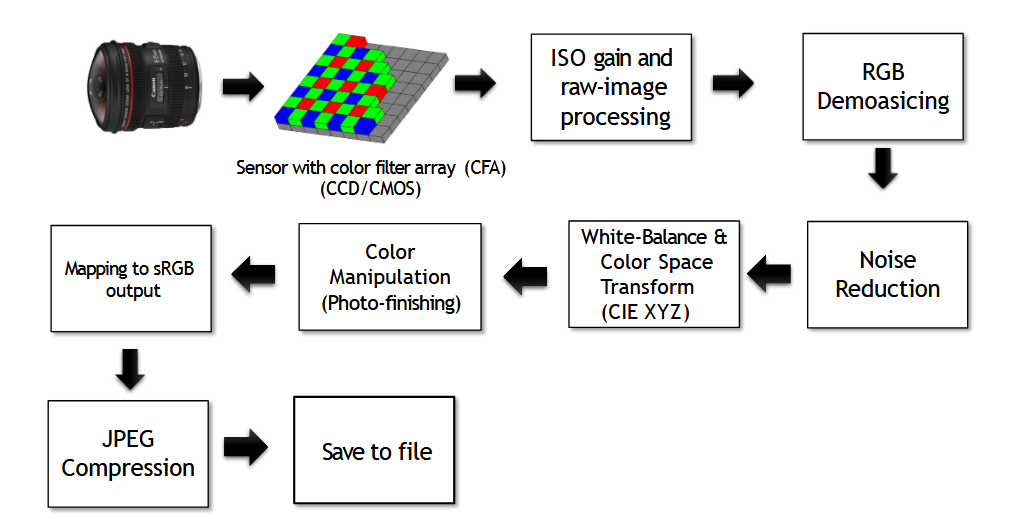
\includegraphics[width=1\linewidth]{How_camera_works_pipeline.png}
    \caption{A typical camera pipeline.
    NOTE: This is an example for a standard consumer camera, there are many other cameras which can have different elements in it. }
    \label{fig:camera_pipeline}
\end{figure}
\noindent
These processes mostly differ from camera to camera, which all have their own distinct methods, hardware, settings and quality. This leads to differences in the final footage, which an example of can be seen in Figure \ref{fig:lens_comparison}, where images have different characteristics all depending on the camera used. It is important to understand these fundamental elements when working with surveillance recordings, as they expose the different factors that influence the final output footage, and the way it is processed and worked on\cite{korene_imatest2022_cv_iq}.
\begin{figure}[H]
    \centering
    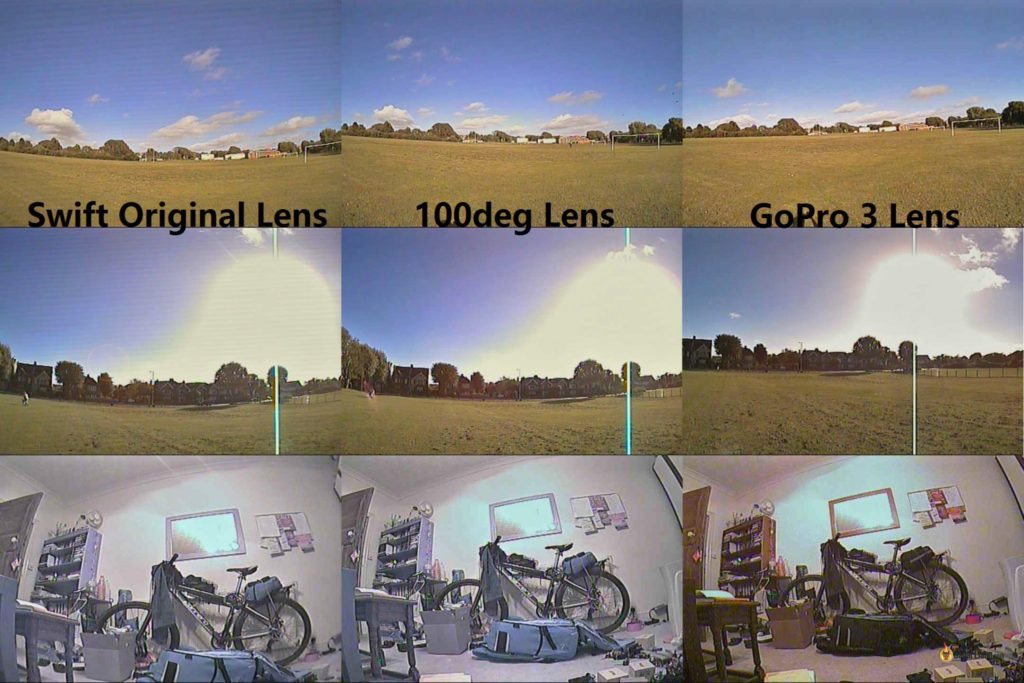
\includegraphics[width=0.7\linewidth]{runcam-swift-lens-comparison.jpg}
    \caption{Lens comparison on different cameras to highlight change in color, brightness and Field Of View (\acs{FOV}) in the footage.}
    \label{fig:lens_comparison}
\end{figure}
\subsection{Technical Impacts on Footage}
As stated in Chapter \ref{subsubsec:How_cameras_work}, there are many different factors that can influence the overall output of the image. The cameras themselves are rarely alike in terms of quality and features, and some also have restrictions on resolution and refresh rate to reduce energy consumption and storage, while others are able to deliver clearer images with higher resolution and smoother frame rates. In addition, certain cameras include extra functionalities such as night vision, infrared (\acs{IR}), or pan tilt-zoom (\acs{PTZ})\cite{nightvision_enhancement2018}. This is important to be aware of when working with Artificial Intelligence (\acs{AI}), as computer vision works by analyzing and learning the different pixel patterns in images and videos\cite{common_challenges_image_class2024}, which, if not done correctly, can cause unwanted biases for the \acs{AI}-model when used on other surveillance systems by fixating on unimportant noise that would not be present in other instances \cite{opencv2025visionproblems}.

\subsection{Environmental Impacts on Footage}
As surveillance cameras are used for many different tasks, they will be placed in a variety of situations and conditions. Just like how the internal hardware and software can cause challenges when using \acs{AI}, the external factors such as location, season, and weather can create difficulties as well. For example, there are a lot of differences in footage from a camera that is placed inside rather than outside where weather like rain or snow can create noise which reduce clarity and usefulness in the final footage. In contrast, a camera inside is not affected by this, and therefore is viewed differently by the model.\cite{arxiv_suerres2021}. 
\\\\
Other aspects that can influence the models ability to generalize is also light. Many surveillance cameras are used at night, where only minimal visibility is created with a spotlight or \acf{IR} filters \cite{nightvision_enhancement2018}. This creates a contrast with cameras that are in well-lit areas, which have no use for these filters.
\\\\
Footage quality also gets worse the greater distance it is recording. As seen in Figure \ref{fig:camera_distance}, subjects further away from the camera get blurrier and more unrecognizable, which is also one of the reasons for implementing a \acf{SR} system, that can create usable data of such cases. 
\begin{figure}[H]
    \centering
    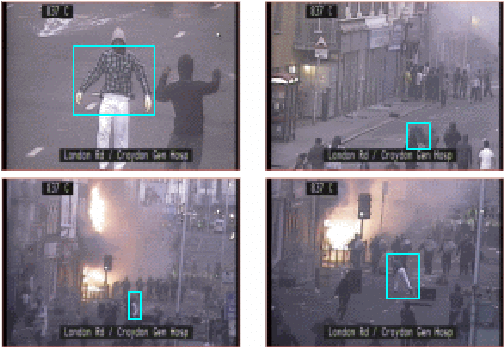
\includegraphics[width=0.7\linewidth]{Typical-images-from-a-single-CCTV-camera-with-poor-lighting-and-long-range-camera-views.png}
    \caption{Picture from a surveillance camera in poor light and different distances to the subject marked with a cyan box.}
    \label{fig:camera_distance}
\end{figure}

\section{Re-identification}

\ac{ReID} is the task of identifying the same person across multiple non-overlapping camera views. Unlike related applications such as face recognition, or tracking movement from a single camera, person \acs{ReID} aims to operate across larger areas that extend beyond the field of view of a single camera. Such a system can be used to track customer behavior in stores, pedestrian traffic in public transport, vulnerable individuals in healthcare facilities, or \ac{POI} for law enforcement. 

\subsection{Re-identification Networks}
Her skal der stå noget om hvad et ReID netværk er. 

\subsection{The Challenges of Re-identification}
As the network must function across multiple non-overlapping camera views, the key challenges are adapting to variations in camera angles, resolution, lighting, background, and partial or full occlusion of the \acs{POI} \cite{IntroPReID2023}.

\subsection{Few-shot Learning}
Furthermore, due to the nature of the task, each person inhabits a unique class that is rarely observed more than once, causing \ac{ReID} to inherently pose a \ac{FSL} problem. The main challenge then becomes designing a pipeline which extracts robust and discriminative features across diverse environments, while also ensuring enough information is kept for \acs{FSL} to be viable.

\section{Super-resolution}

\ac{SR} denotes the reconstruction of a \ac{HR} image or video frame sequence from one or more \ac{LR} observations. Because many different \acs{HR} images can downsample to the same \acs{LR} input, \acs{SR} is an ill-posed inverse problem; practical systems therefore rely on learned priors to constrain the solution space. Deep learning has reshaped \acs{SR} by learning an end-to-end mapping from \acs{LR} to \acs{HR} directly from data. A seminal example is SRCNN, which established that a compact \ac{CNN} can outperform hand-crafted pipelines by regressing \acs{HR} images from bicubic-upsampled \acs{LR} inputs, demonstrating the viability of supervised, data-driven \acs{SR}.\cite{dong2015imagesuperresolutionusingdeep}

\subsection{Deep Learning Approaches}

Modern \acs{SR} models extend this idea with deeper networks, residual connections, perceptual losses, and adversarial training. GAN-based methods such as ESRGAN optimize not only for low pixel-wise error but also for visual realism as perceived by humans, introducing architectural refinements (e.g., Residual-in-Residual Dense Blocks) and improved loss formulations to generate sharper, more natural textures. These advances pushed \acs{SR} beyond “blurry but accurate” predictions toward photo-realistic reconstructions useful for visual consumption and media upscaling \cite{Wang2019ESRGAN}.

\subsection{Perception–distortion trade-off and evaluation}

A central insight for \acs{SR} system design is the formalized perception–distortion trade-off: minimizing distortion metrics (e.g., PSNR/SSIM) and maximizing perceptual quality cannot be optimized simultaneously. Consequently, objective choice restoration fidelity for scientific/forensic analysis versus perceptual realism for display should drive loss selection and model configuration. Evaluations typically report both distortion measures and perceptual assessments (learned perceptual metrics or human studies) to position a method on this trade-off curve \cite{Blau2018PerceptionDistortion}.

\section{Super-resolution Re-identification}
